\chapter{Facilitating re-interpretation} % 
\label{cha:simplifiedLikelihood}
The results of the \alphat search have been presented using limits on simplified model
spectra which allow the sensuality of the search to different topologies 
to be benchmarked. The search will be sensitive to a wide range of BSM models
and the results must therefore be re-interpreted by those outside the 
CMS collaboration to provide constraints on such models.

The \alphat search, like many searches for BSM physics with the CMS detector, uses a 
fine categorisation to separate background from signal contributions. To re-interpret
such a search the signal yield is typically evaluated using an event generator such as \PYTHIA 
followed by a simulation of the detector response and resolution using tools 
such as \DELPHES~\cite{delphes} or using published efficiencies for generator
level quantities (both methods are used in~\cite{Drees:2013wra,Fastlim,mastercode}).
The background contributions to the search regions and the associated systematic uncertainties often rely
on simplifying assumptions which can lead to inaccuracies in the re-interpretation. 

In this section an alternative procedure for re-interpreting BSM physics searches by approximating
the full background model and the associated systematic uncertainties is presented. 
The procedure involves techniques both to simplify the categorisation of the search (\emph{aggregation})
and to use a reduced set of information to describe the background model 
and the correlations between different search regions (\emph{simplified likelihood}),
minimising the loss of sensitivity. The \alphat search is used to validate and illuminate
the use of such techniques, however, they are applicable for a wide range of 
searches and a general treatment may be found in~\cite{simp-lik}.

\section{Aggregation}%
\label{sec:agg-reg}
The \alphat analysis uses a fine categorisation in \njet, \nb, \scalht,and \mht to provide
sensitivity to a wide range of new physics models. This categorisation makes re-interpreting
the results of the search too computationally intensive to be feasible. Previously, 
only the categories most sensitive to the relevant model have been used, however,
this will break the correlation model for the search and can significantly reduce
the sensitivity due to the loss of indirect constraints from
the neglected bins. 

In this section, the definition of aggregated regions 
using the full likelihood is presented. The aggregated regions allow the categorisation to be 
simplified without breaking the background model. 

\subsection{The aggregate region likelihood}

Consider the hadronic component of the likelihood defined in Equation~\ref{eq:hadronicLikelihood}.
The aggregate likelihood is defined by summing the contributions within the Poisson for
each \mht, \scalht, \nb and \njet category to be aggregated as,

\begin{multline}
\label{eq:aggregatedLikelihood}
\mathcal{L}^{\text{agg}}_{\mathrm{had}} = \prod_{\text{agg}_{k}} {L}^{\text{agg}_{k}}_{\mathrm{had}} = \mathrm{Pois}(\sum_{i,j\in\text{agg}_{k}} n^{j,i}_{\mathrm{had}} |\sum_{i,j\in\text{agg}_{k}}\, b^{j,i}_{\zInv~,had}\times\phi^{j}(\mu\rightarrow\zInv~)\times a^{j}\times\rho^{j,i}_{\zInv~,had}\, + \\ 
b^{j,i}_{\ttW,\mathrm{had}}\times\phi^{j}(\mu\rightarrow\ttW)\times a^{j}\times\rho^{j,i}_{\ttW,had}\, + b^{j,i}_{\text{QCD},had}\times\omega^{j,i}_{\text{QCD},had}\\\
+ \,r\times s^{j,i}_{\mathrm{had}}\times\rho^{j,i}_{s,had}).
\end{multline}

The control region component of the likelihood is unchanged such that the prediction model
is maintained from the full likelihood. This allows, for example, the scale anchoring 
scheme to maintain validity while allowing events at different scales to be included 
within the same aggregate region.

\subsection{Definition of aggregated regions}
\label{sec:ssr-alphat}
The categorisation used for the full likelihood is summarised in Section~\ref{sec:cat}. 
The large number of categories provide generic sensitivity but are not optimal for re-interpretation. 
The thirty one jet categories are therefore reduced to eight aggregate jet categories while
the (up to) eight \scalht bins are merged into one ($\scalht \geq 200 GeV$).
The final categories are shown in Table~\ref{tab:agg-binning}.
These are defined to be disjoint, contiguous and to cover the full
signal region such that in combination the regions reflect the sensitivity of
full signal region phase space.

\begin{table}[htb!]
  \caption{To define the aggregate regions for the \alphat search the \scalht dimension is
  merged to $\geq200\GeV$ and $\nb$ to two categories of \nb~$<2$ and $\geq2$. 
  The merged \nj~ categories are summarised in this table. Each category is
  further binned using eight \mht bins with lower bounds from $100-800\GeV$.}
  \label{tab:agg-binning}
  \centering
  \footnotesize
  \begin{tabular}{ llll }
    \hline
    \nj~topology & \multicolumn{3}{l}{Merged jet categories} \\
    \hline
     & \bf Monojet & \bf Asymmetric& \bf Symmetric \\
    Monojet-like & 1 & 2 & 2                         \\
    Asymmetric high \nj& - & 3, 4, $\geq5$ & -                 \\
    Mid \nj & - & - & 3, 4                         \\
    High \nj & - & - & $\geq5$                      \\
    \hline
  \end{tabular}
\end{table}

The jet categories are merged to four seperate categories motivated by their sensitivity to 
different new physics topologies. For example, the Monojet-like topology is targeted towards
dark matter models and compressed spectra while the high \nj topology targets 
uncompressed gluino and squark models. The \nb categories are combined 
as $\nb=0,1$ and $\nb\geq2$ targeted at light and heavy flavour new physics respectively. 
Finally, the \scalht dimension is entirely merged as the \mht dimension generally provides better sensitivity
for new physics models. The use of the aggregated regions ensures that the backgrounds are 
still predicted by the nominal, finely binned regions (with appropriate systematics).

\subsection{Results using aggregated regions for the \alphat analysis}

The aggregated regions provide an easily comprehensible
overview of the signal region when compared to the results
of the nominal signal bins. Figure~\ref{fig:aggFitResult} shows
the post fit predictions in the mid and high \nj categories
for the aggregated regions compared to the observed data.

\clearpage
\begin{figure}[!tbhp]
    \caption{ Signal region predictions and data observations for the aggregated regions. 
    The predictions are made using a fit to the control region only. \label{fig:aggFitResult} }
  \begin{center}
    \subfigure[Mid \nj, $\nb \leq 1$]   { 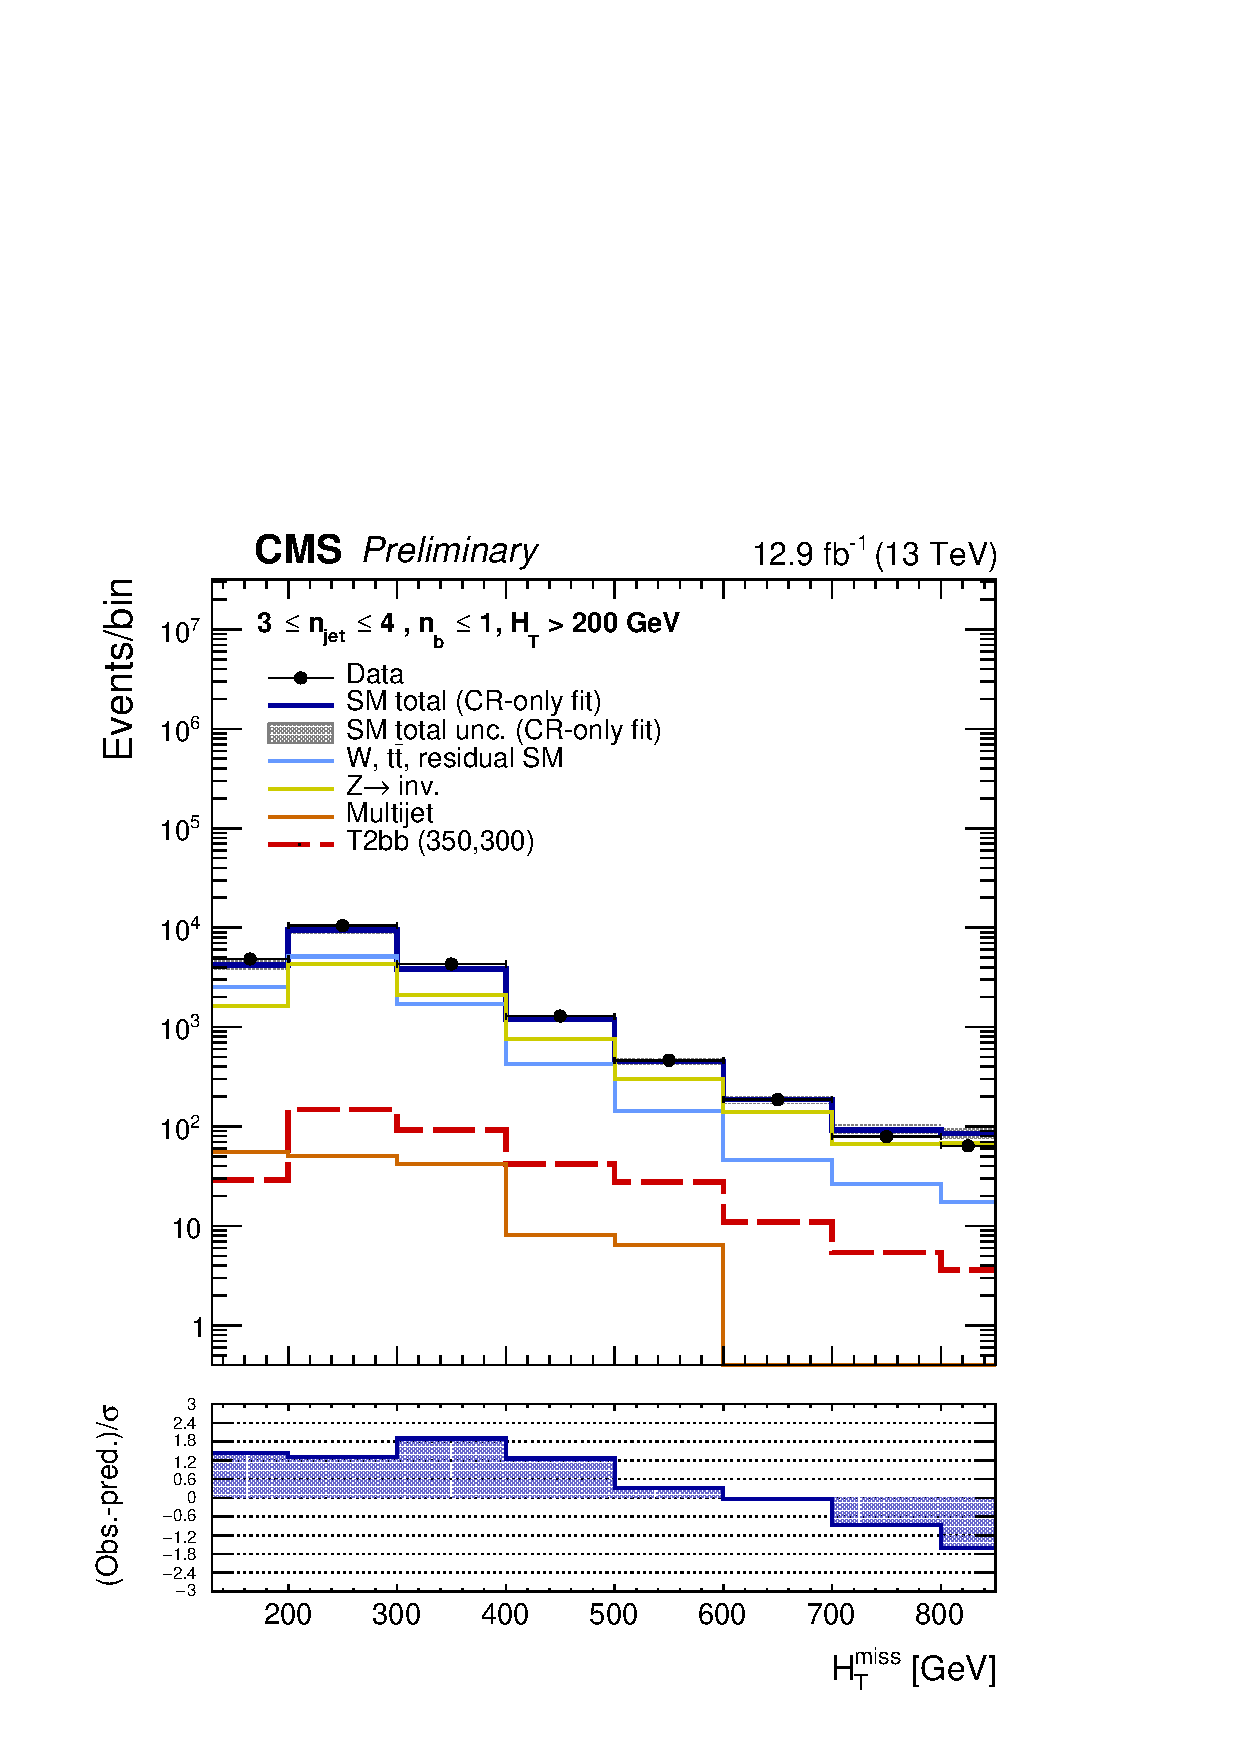
\includegraphics[width=0.45\textwidth]{Figures/simplifiedLikelihood/agg_fitResults/mhtShape_le1b_ge3j_200_Inf_crfit_aux.pdf} } ~~
    \subfigure[Mid \nj, $\nb \geq 2$]{ 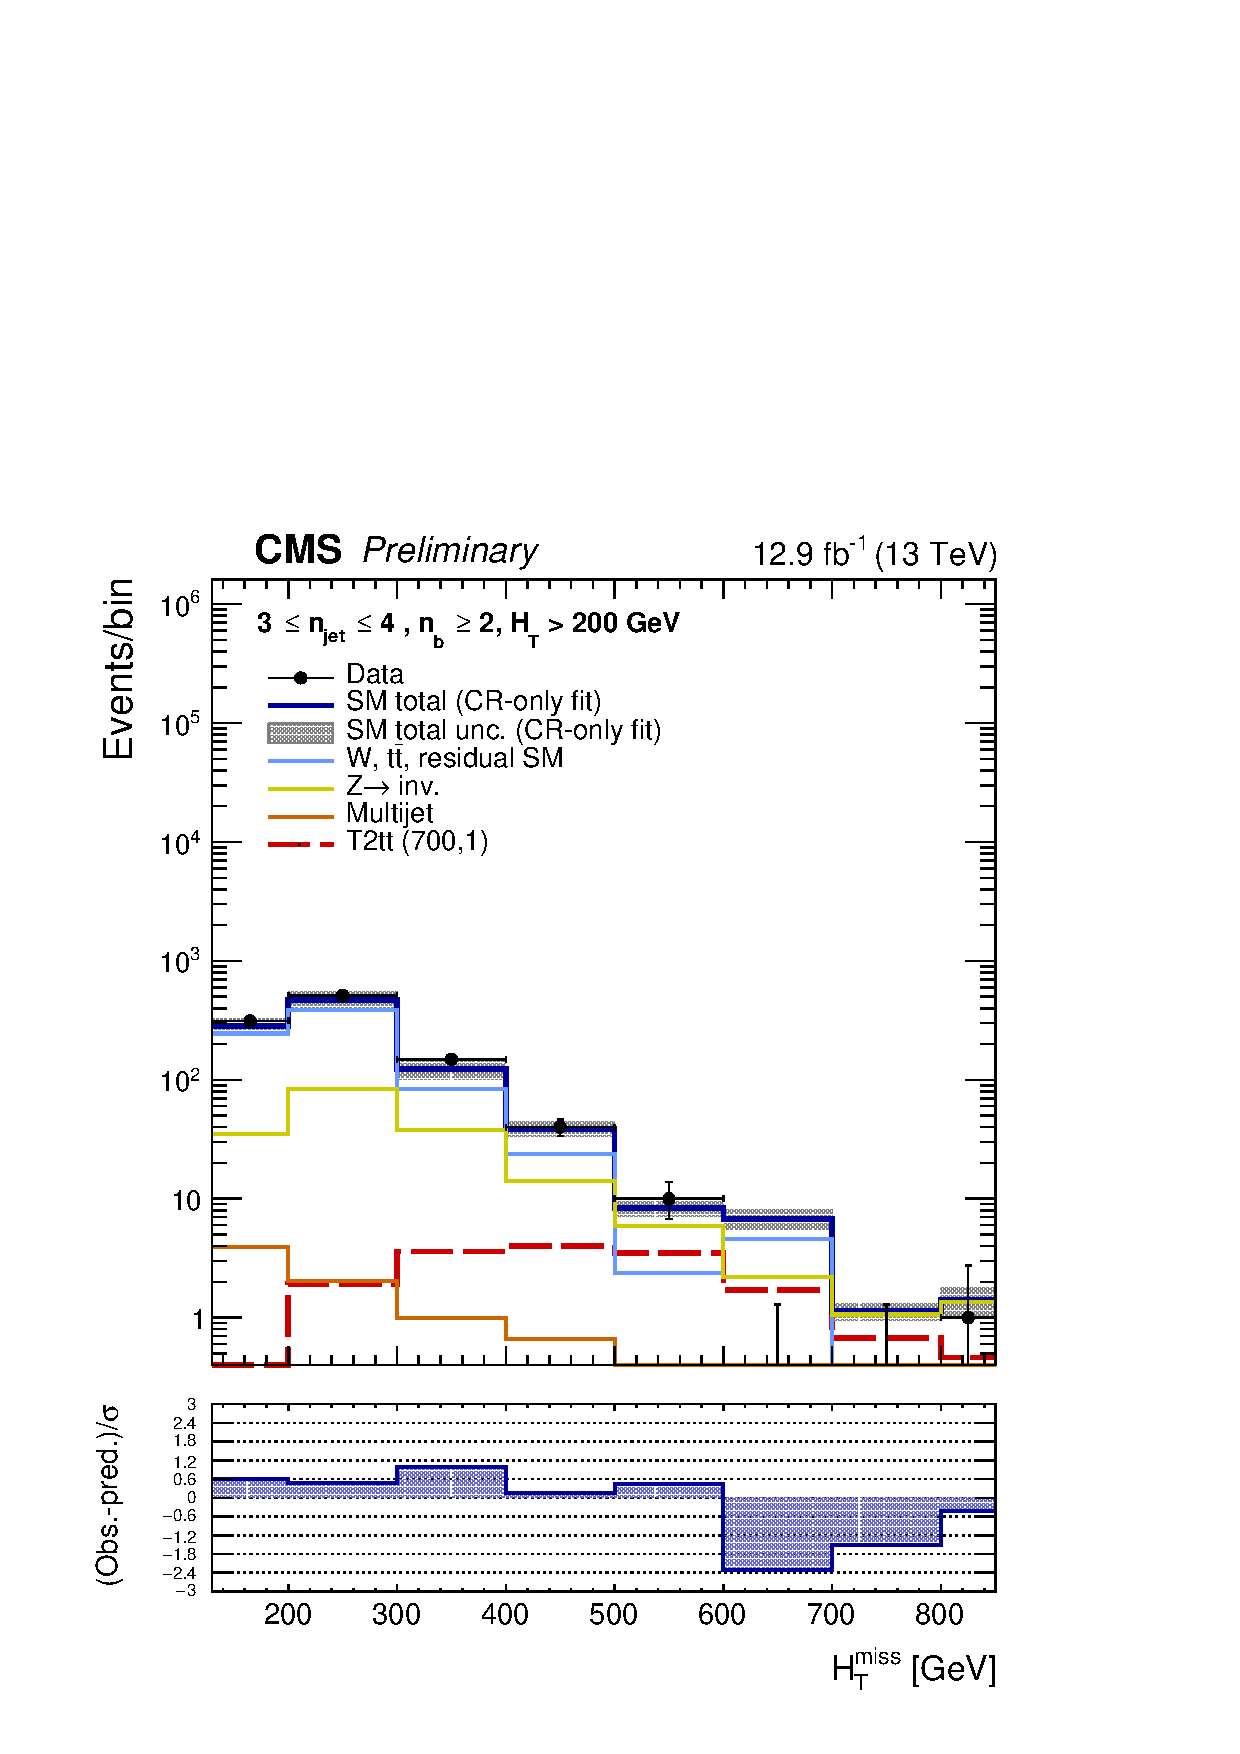
\includegraphics[width=0.45\textwidth]{Figures/simplifiedLikelihood/agg_fitResults/mhtShape_ge2b_ge3j_200_Inf_crfit_aux.pdf} } \\
    \subfigure[High \nj, $\nb \leq 1$]   { 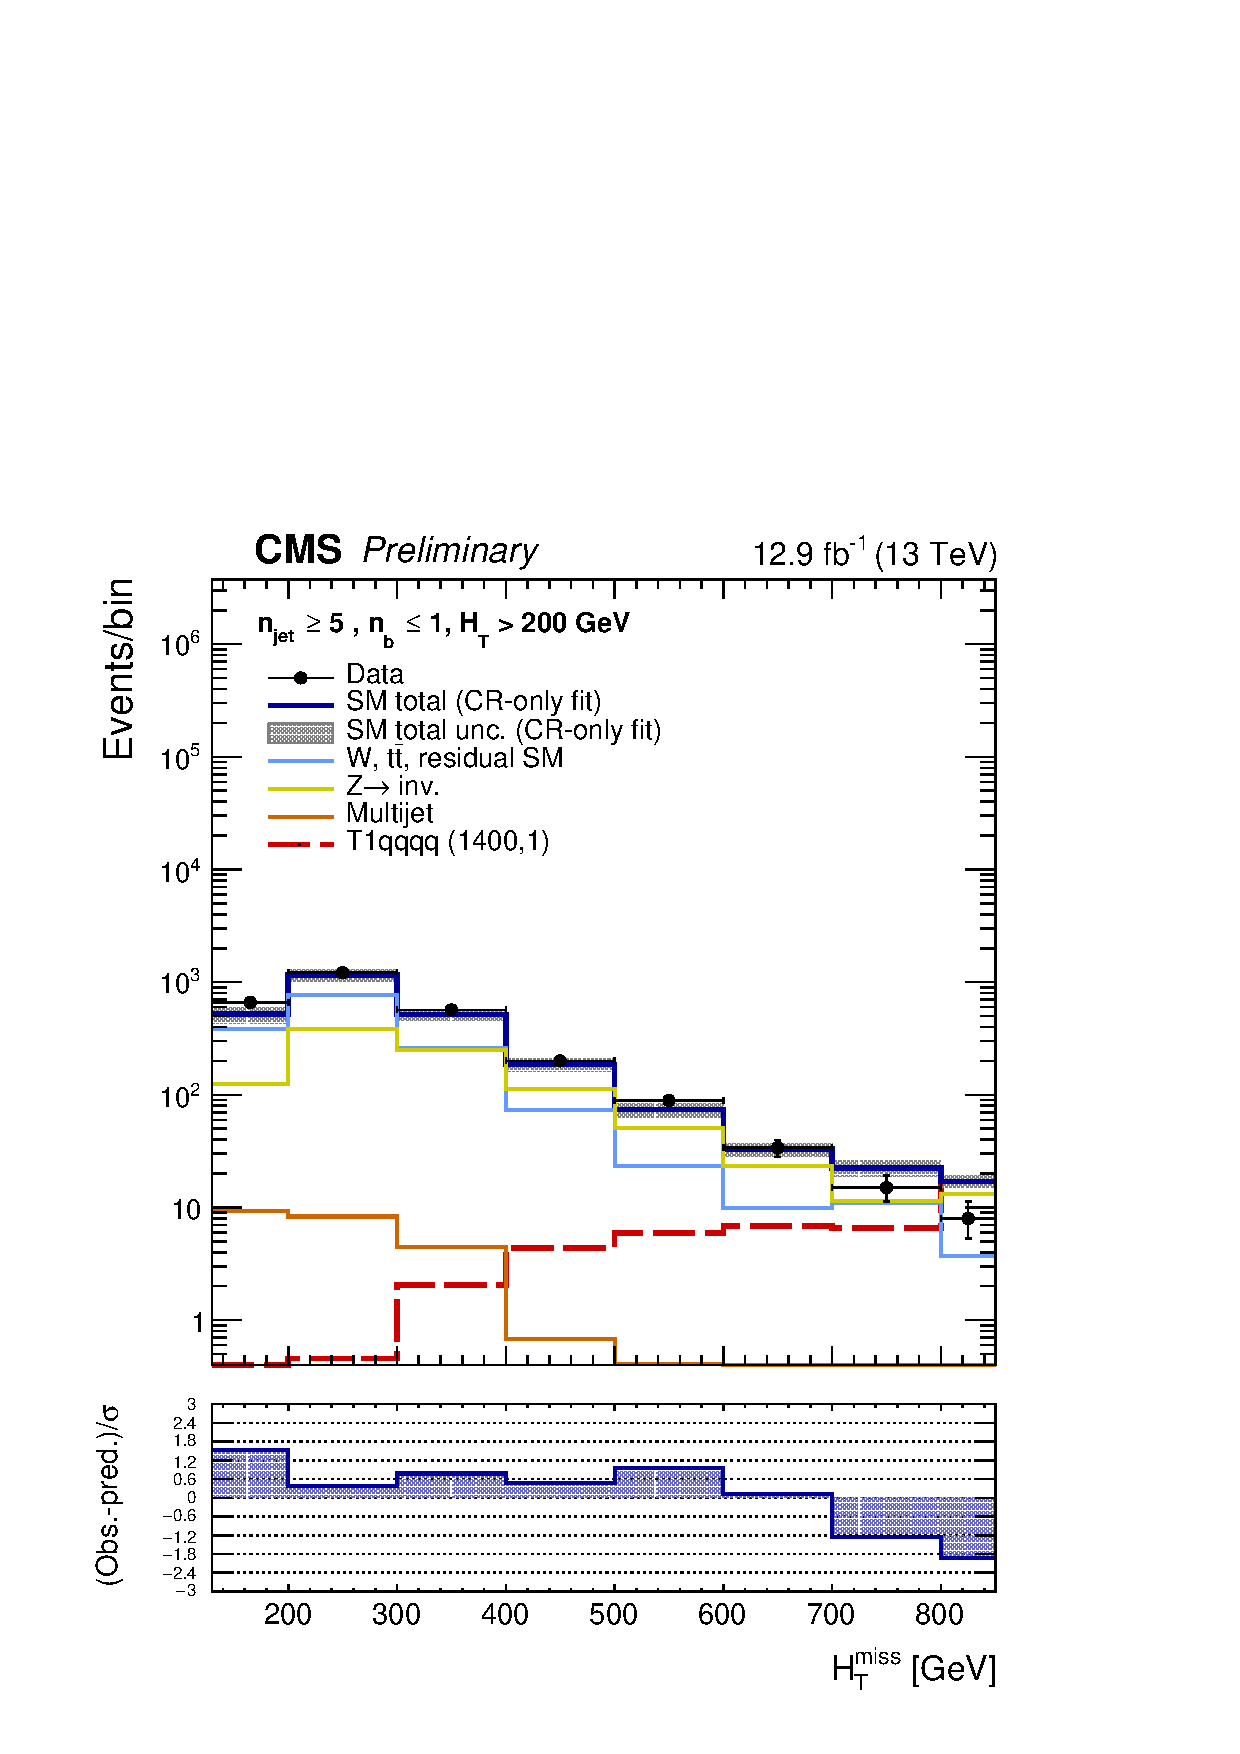
\includegraphics[width=0.45\textwidth]{Figures/simplifiedLikelihood/agg_fitResults/mhtShape_le1b_ge5j_200_Inf_crfit_aux.pdf} } ~~
    \subfigure[High \nj, $\nb \geq 2$]{ 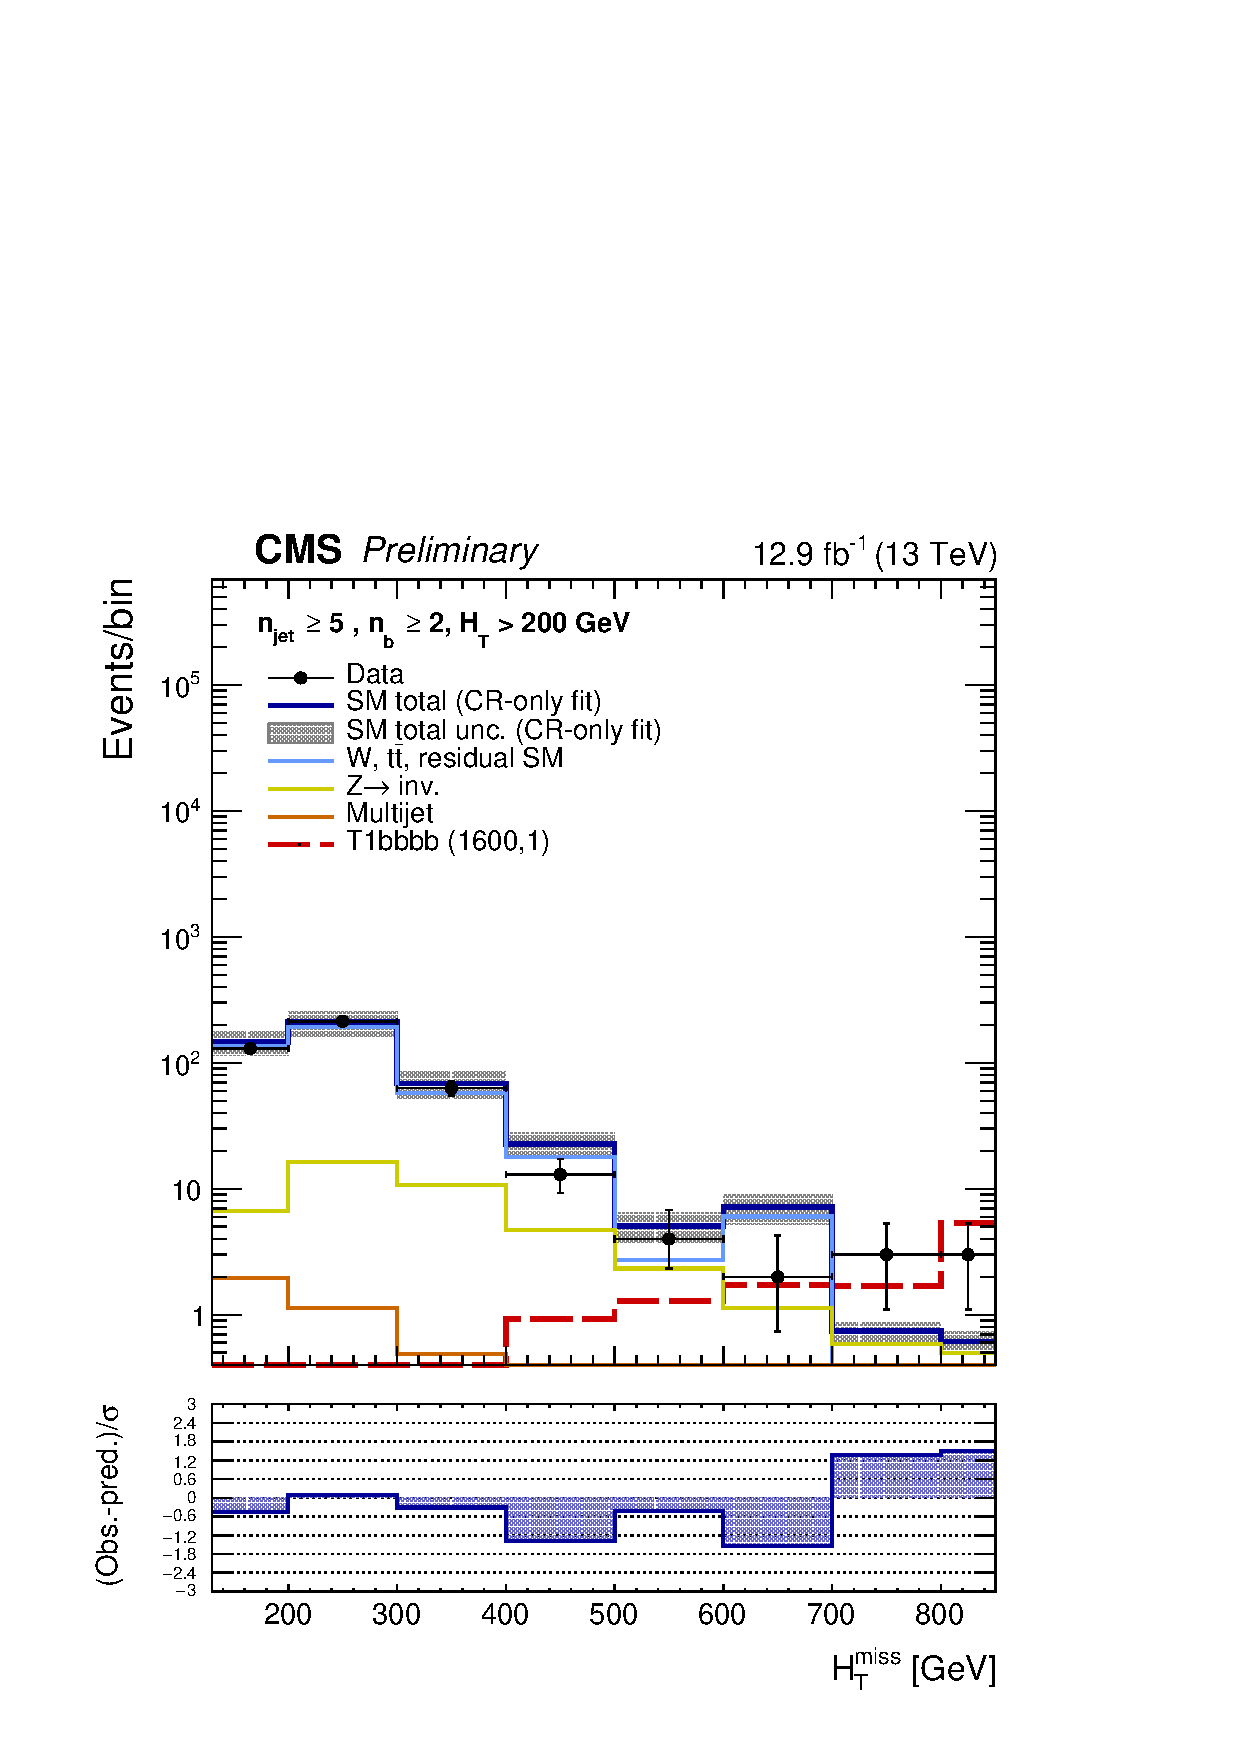
\includegraphics[width=0.45\textwidth]{Figures/simplifiedLikelihood/agg_fitResults/mhtShape_ge2b_ge5j_200_Inf_crfit_aux.pdf} } \\
  \end{center}
\end{figure}

To evaluate the effect on the sensitivity of the \alphat analysis of using
the aggregated regions the expected and observed 95\% upper limit
on the signal strength for the full signal region 
is compared to the limits derived using the aggregated regions. The limits are shown side by side
in Fig~\ref{fig:limit-planes-agg} for three models, T2tt T2bb and T1bbbb. Where the mass
splittings are small the expected limits typically reduce by $\mathcal{O} 100\GeV$ 
compared to the full signal region.

\clearpage
\begin{figure}[!tbhp]
    \caption{Limit planes shown for both the full signal regions (left) and the aggregated regions (right).\label{fig:limit-planes-agg}.}
  \begin{center}
    \subfigure[T2bb full signal region]{ 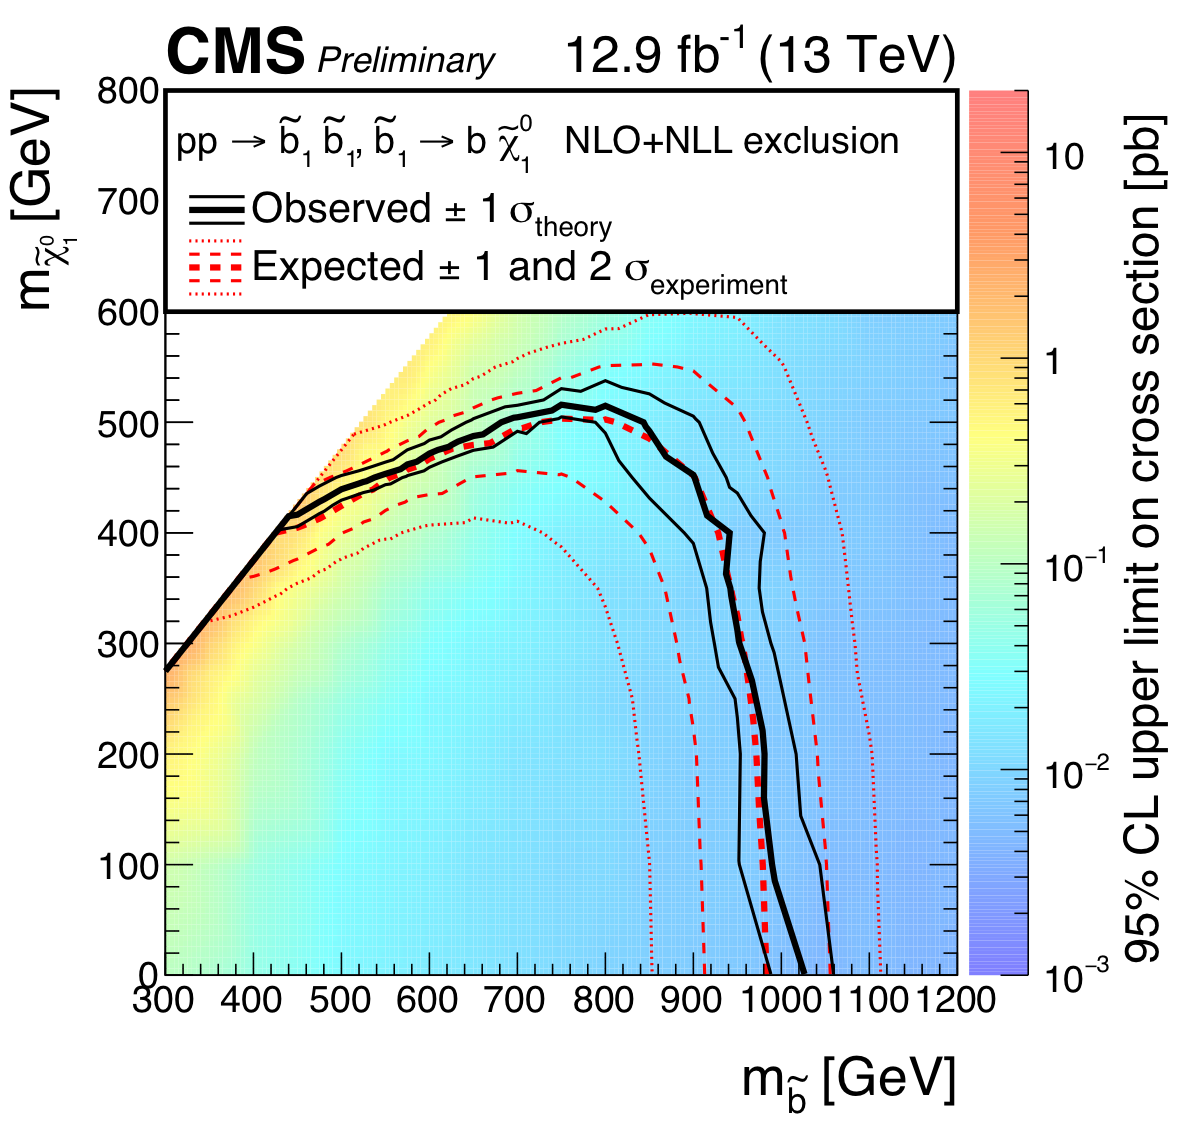
\includegraphics[width=0.45\textwidth]{Figures/simplifiedLikelihood/limitPlanesNominal/SUS16T2bbXSEC.png} } ~~
    \subfigure[T2bb aggregated regions]{ 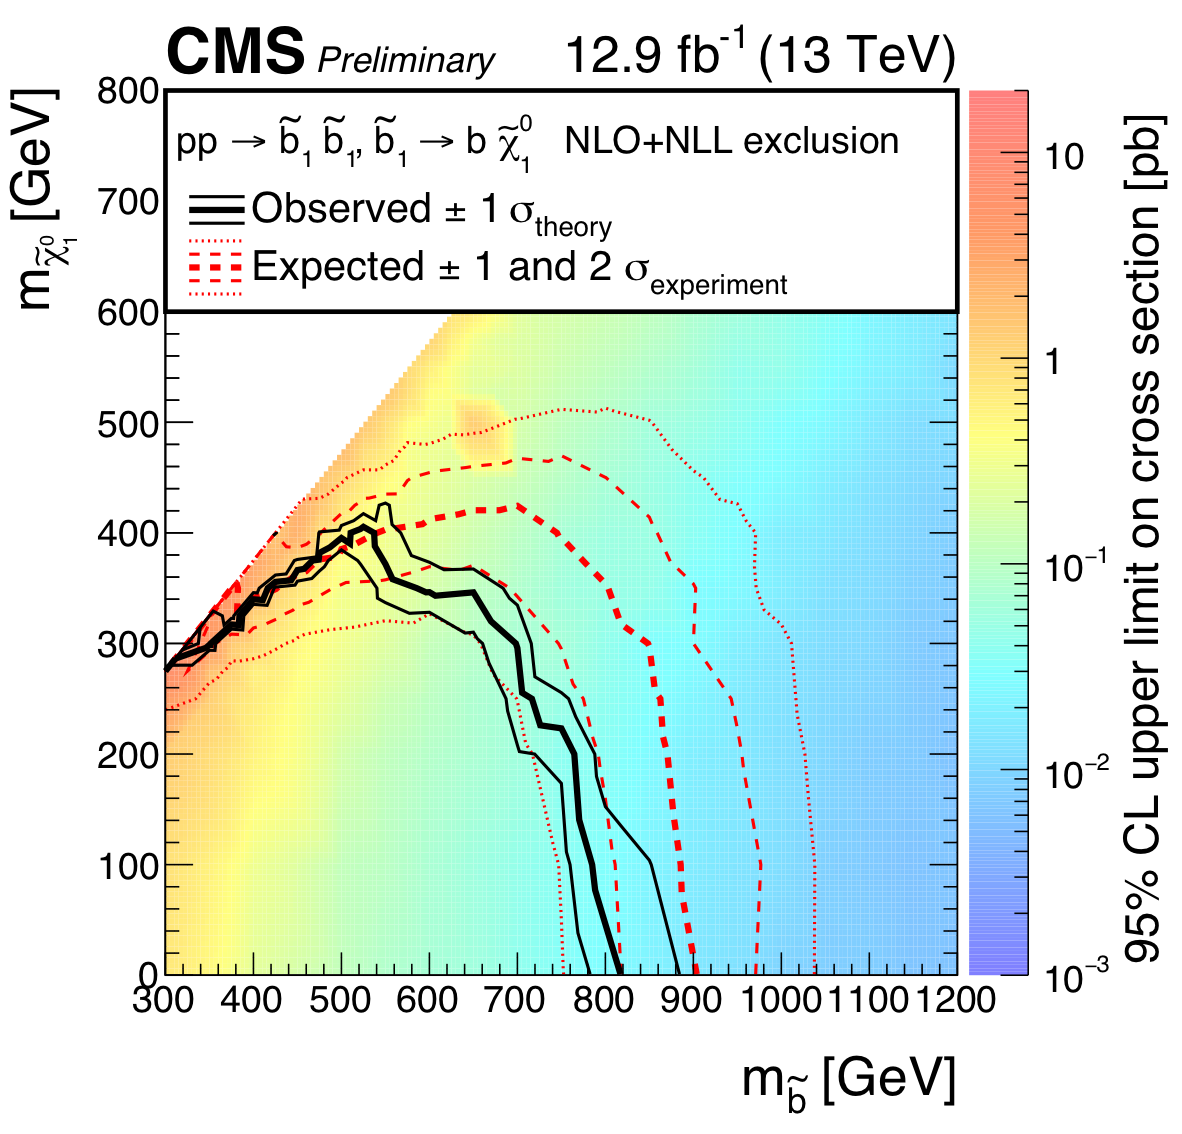
\includegraphics[width=0.45\textwidth]{Figures/simplifiedLikelihood/limitPlanesAgg/SUS16T2bbXSEC.png} } \\
    \subfigure[T2tt full signal region]   { 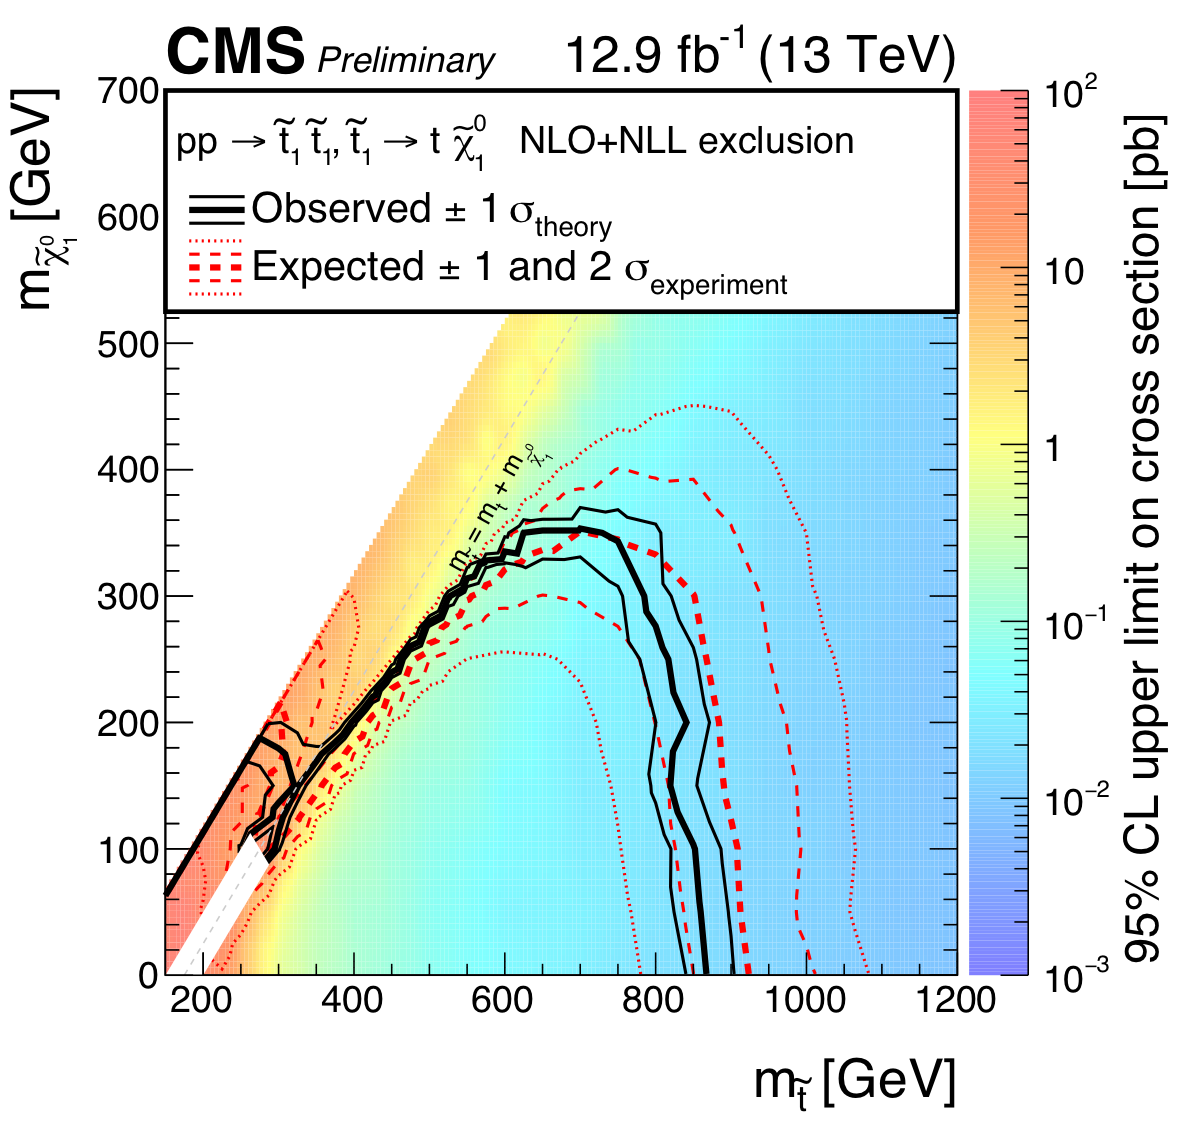
\includegraphics[width=0.45\textwidth]{Figures/simplifiedLikelihood/limitPlanesNominal/SUS16T2ttXSEC.png} } ~~
    \subfigure[T2tt aggregated regions]{ 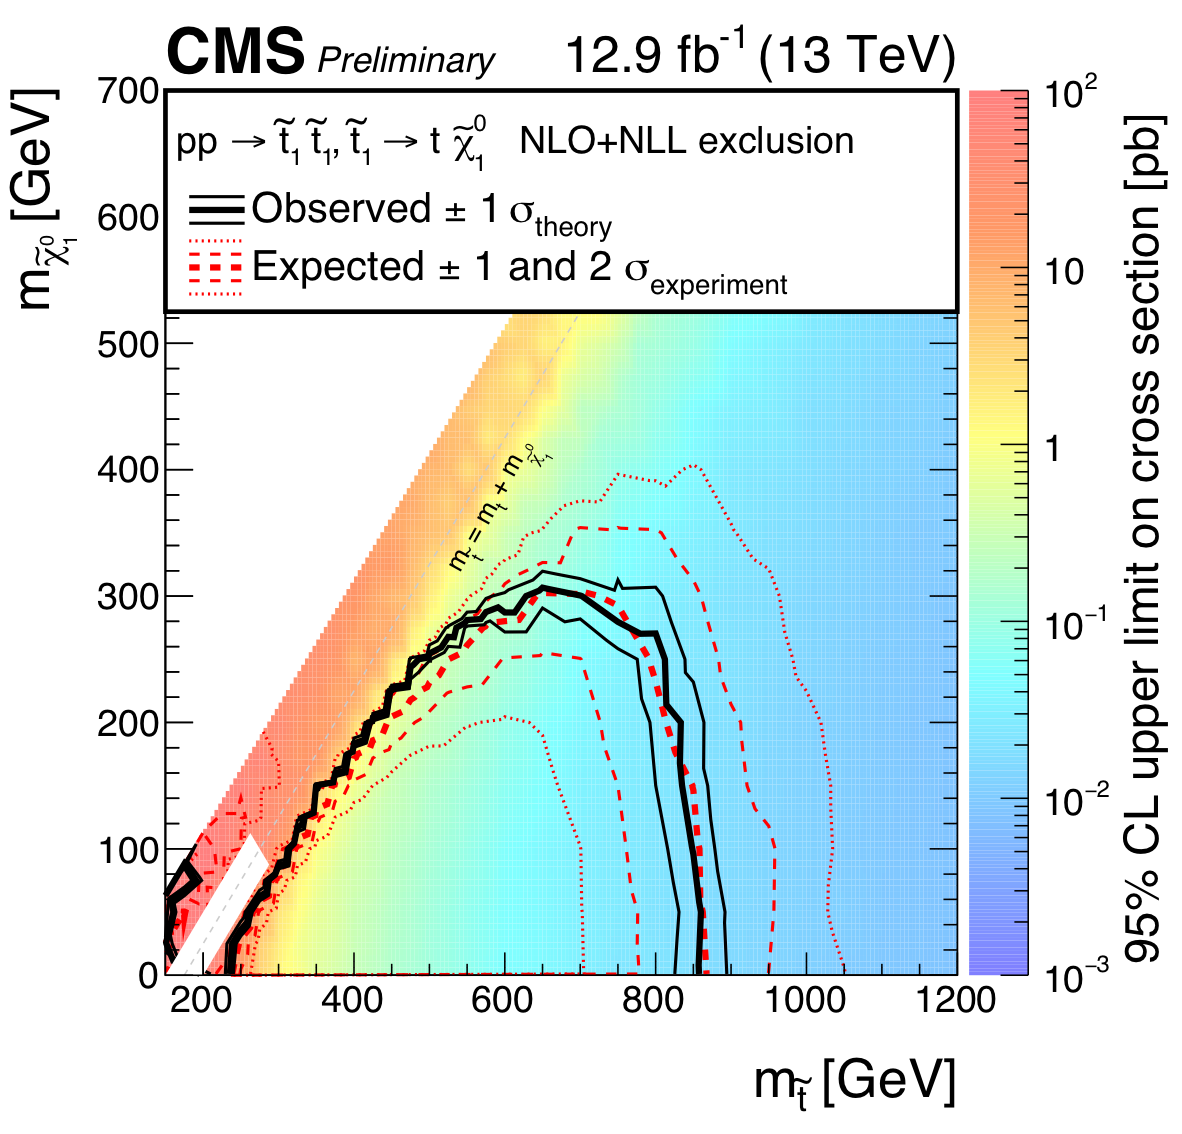
\includegraphics[width=0.45\textwidth]{Figures/simplifiedLikelihood/limitPlanesAgg/SUS16T2ttXSEC.png} } \\
    \subfigure[T1bbbb full signal region]   { 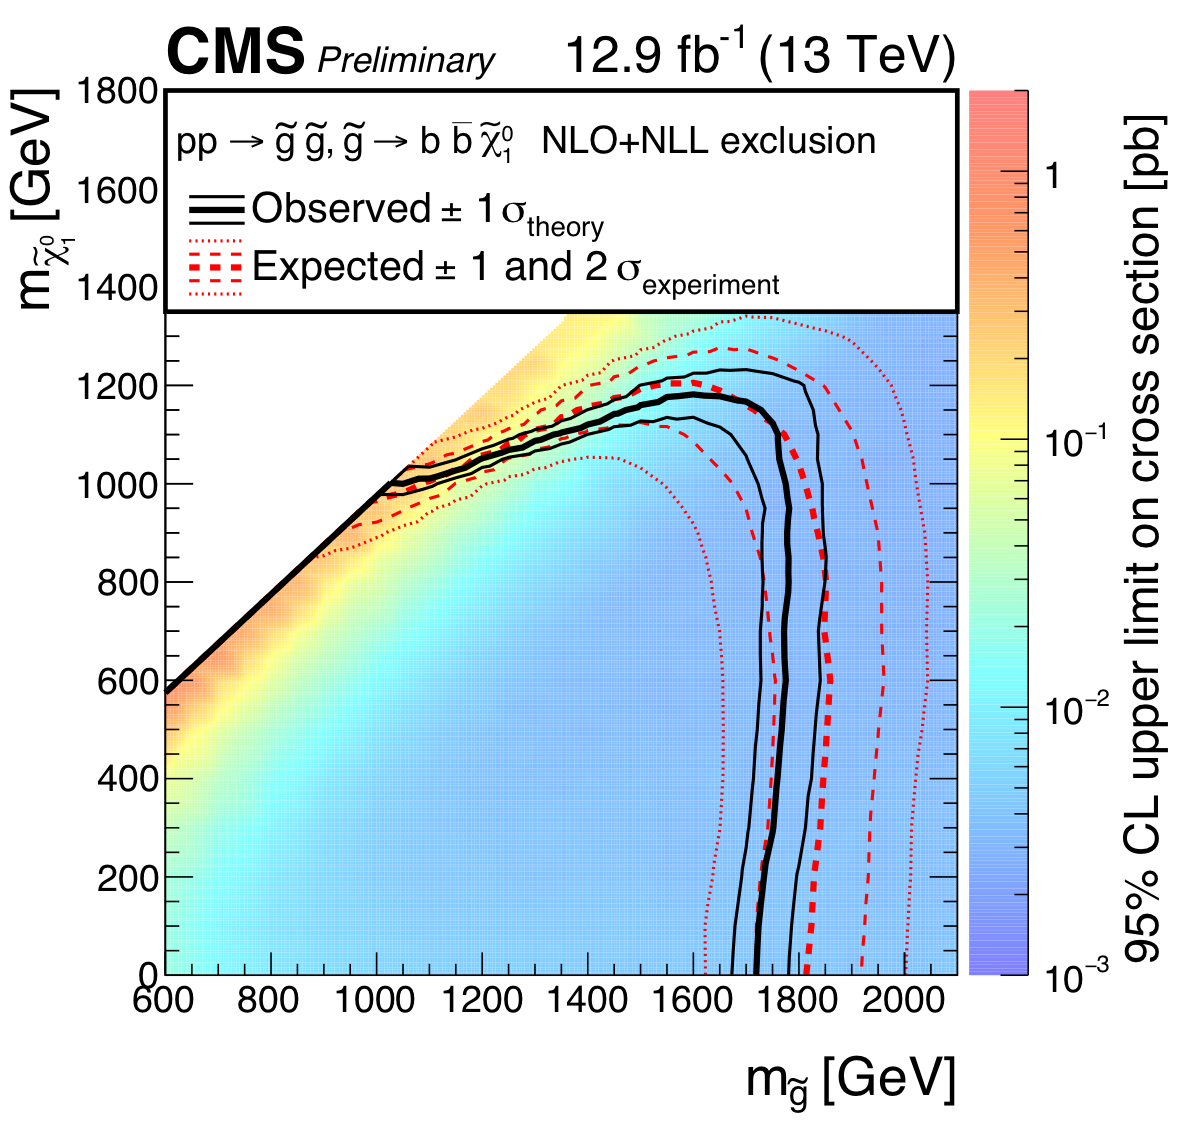
\includegraphics[width=0.45\textwidth]{Figures/simplifiedLikelihood/limitPlanesNominal/SUS16T1bbbbXSEC.png} } ~~
    \subfigure[T1bbbb aggregated regions]{ 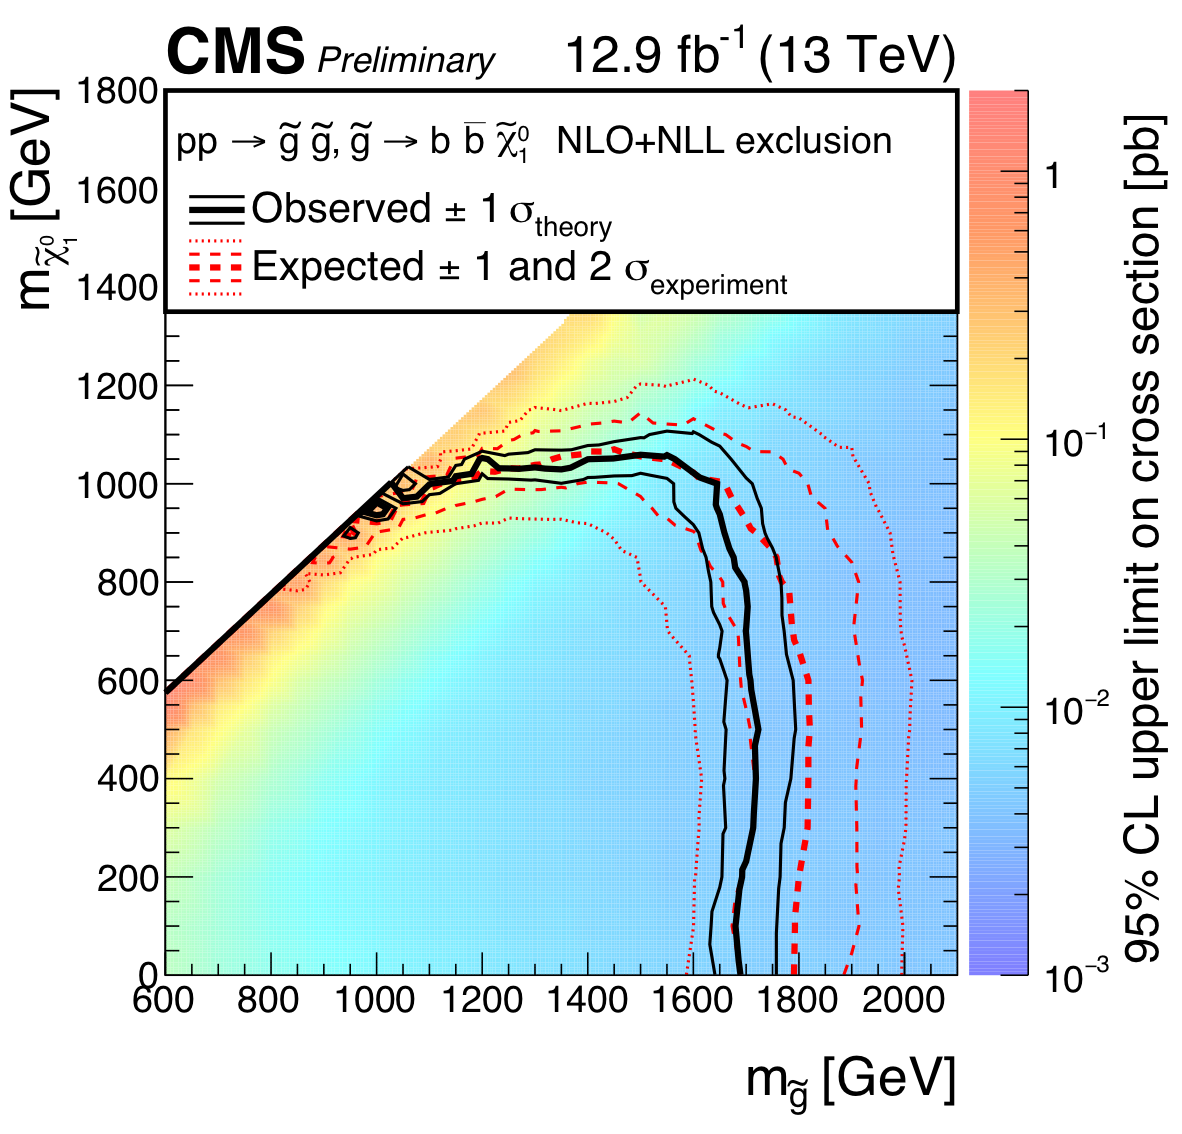
\includegraphics[width=0.45\textwidth]{Figures/simplifiedLikelihood/limitPlanesAgg/SUS16T1bbbbXSEC.png} } \\
  \end{center}
\end{figure}

\section{Simplified likelihood}

In this section a method for simplifying the likelihood by approximating the nuisance parameters
using a multivariate Gaussian is described. The approximations and areas of applicability 
are made are discussed and a validation shown using the \alphat~search.

\subsection{Definition of the simplified likelihood}

The form of the likelihood (either aggregate or full) used by the \alphat~analysis (product of poisson terms 
for the observation in each bin given the prediction and uncertainties)
is typical for searches for BSM physics. Neglecting uncertainties on the signal contribution,
the likelihood may be written as 

\begin{equation}
\mathcal{P}(\mathrm{data}|\mu\cdot s(\boldsymbol{\theta}) + b(\boldsymbol{\theta})) = \prod_{i=1}^{N} P(n_{i}|\mu \cdot s_{i}+b_{i}+\theta_{i}).
\label{eq:poisson-prob}
\end{equation}

where the product is over all categories (with total N) and all nuisance parameters
have been included in the absolute variation in the total background, $\theta_i$. The simplified likelihood 
is the approximation of the full probability density function $p(\tilde{\boldsymbol{\theta}}|\boldsymbol{\theta})$
as a multivariate Gaussian using the covariance between the categories. This approximation relies 
on the following (as detailed in~\cite{simp-lik}):
%Remove and cite????
\begin{itemize}
\item{The constraints on the background contributions are Gaussian such that the distribution of 
the total number of background events is symmetric about the expectation, $b_{i}$, 
with a variance independent of $\boldsymbol{\theta}$. For the \alphat search, as for many analyses, 
this assumption is valid as the background contributions are estimated using control regions in 
data with large sample sizes.}

\item{The covariance, and therefore only the linear correlation, 
between the background contribution in each region is sufficient 
to approximate $p(\tilde{\boldsymbol{\theta}}|\boldsymbol{\theta})$ 
at least for values of $\boldsymbol{\theta}$ which are close to $\tilde{\boldsymbol{\theta}}$.}

\item{The systematic uncertainties in the signal model can be neglected. The validity of 
this assumption will strongly depend on the specific BSM physics model being considered. 
Systematic uncertainties on the signal could be accounted for by adding appropriate 
nuisance parameters with Gaussian constraints (as for the background contributions), however,
their derivation is not feasible for those outside the collaboration.} 
\end{itemize}

Under these assumptions, $p(\tilde{\boldsymbol{\theta}}|\boldsymbol{\theta})$ can be modelled as a multivariate 
Gaussian distribution with the mean vector identified with external measurements of 
$\tilde{\boldsymbol{\theta}}=0$. The simplified likelihood can now be expressed as

\begin{equation}
\mathcal{L}_{S}(\mu, \boldsymbol{\theta}) =  \prod_{i=1}^{N} \dfrac{(\mu \cdot s_{i}+b_{i}+\theta_{i})^{n_{i}} e^{-(\mu \cdot s_{i}+b_{i}+\theta_{i})} }{n_{i}!} \cdot  
\mathrm{exp}\left(-\dfrac{1}{2} \boldsymbol{\theta}^{T}\mathrm{\mathbf{V}}^{-1}\boldsymbol{\theta} \right),
\label{eq:full-likelihood}
\end{equation}

where $\mathrm{\mathbf{V}}$ represents the covariance matrix for the expected background 
contributions across the search regions and is defined as

\begin{equation}
V_{ij}=E[\theta_i\times\theta_j],
\label{eq-cov}
\end{equation}

where $E[x]$ is the expectation value of $x$. The expectations and covariance
must be derived following the fit over the control regions as these are not
included when re-interpreting the search. The covariance matrix is determined
using pseudo-experiments to sample the nuisance parameters. 

As shown in~\cite{simp-lik}, the covariance matrix may also be used to
combine categories into aggregated regions with appropriate covariance between
the bins. These aggregated regions and covariance may then be used to define 
the simplified likelihood.

\subsection{Results for the \alphat~analysis}

The covariance and predictions in the aggregated regions discussed
in Section~\ref{sec:agg-reg} are used to define and validate the simplified likelihood. 
Figure~\ref{fig:likelihoodscanAT} (a) shows the value of $q(r)$ as a function of r for 
a simplified model with direct bottom squark production and $m_\text{SUSY} = 800 \gev$ 
and $m_{\chiz} = 200 \gev$. The values of $q(r)$ are compared to those derived using the full likelihood and 
using the simplified likelihood, ignoring correlations between the background expectations. 
The results using an Asimov dataset, assuming a signal strength of $r=1$, are also 
shown as these are used to calculate limits using the asymptotic approximations 
detailed in Ref.~\cite{Cowan:2010js}. The simplified likelihood,
considering correlations, is shown to be in good agreement with the full likelihood while
the agreement is worsened when correlations are neglected.

In Figure~\ref{fig:likelihoodscanAT} (b) the ratio between the observed $r_{95}$ for the simplified 
and the full likelihood is shown in the ($m_{\text{SUSY}}$, $m_{\tilde{\chi}^{0}}$) plane for 
the simplified model of direct production of bottom squarks. The expected and observed contours of $r=1$ 
excluded at $95\%$ for the full likelihood, the simplified likelihood and the 
simplified likelihood where correlations are neglected are overlaid. The results using the 
full and simplified likelihoods are seen to agree well when the correlations between bins are considered.

\begin{figure}[hbt]
  \begin{center} 
   \subfigure[]{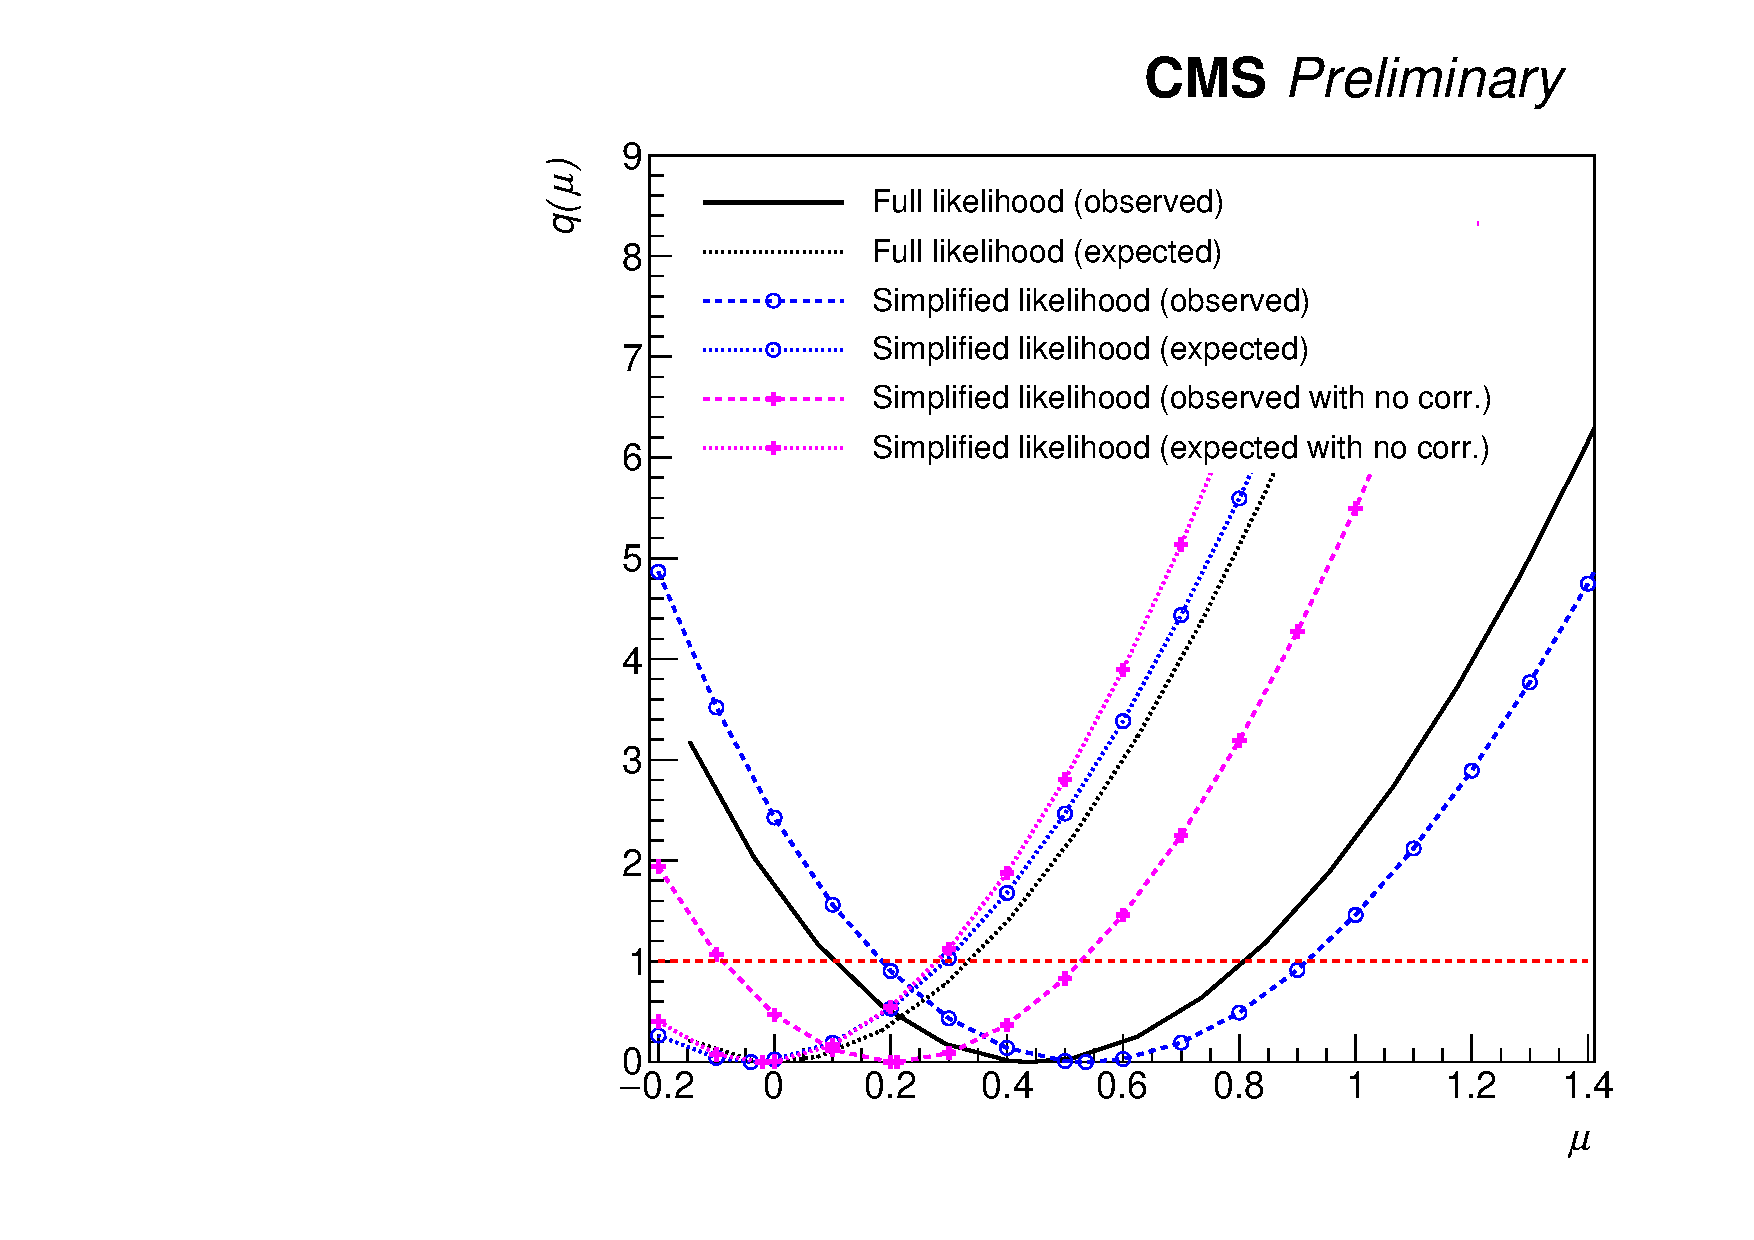
\includegraphics[width=0.45\textwidth]{Figures/simplifiedLikelihood/simpResults/rAT.pdf}}
   \subfigure[]{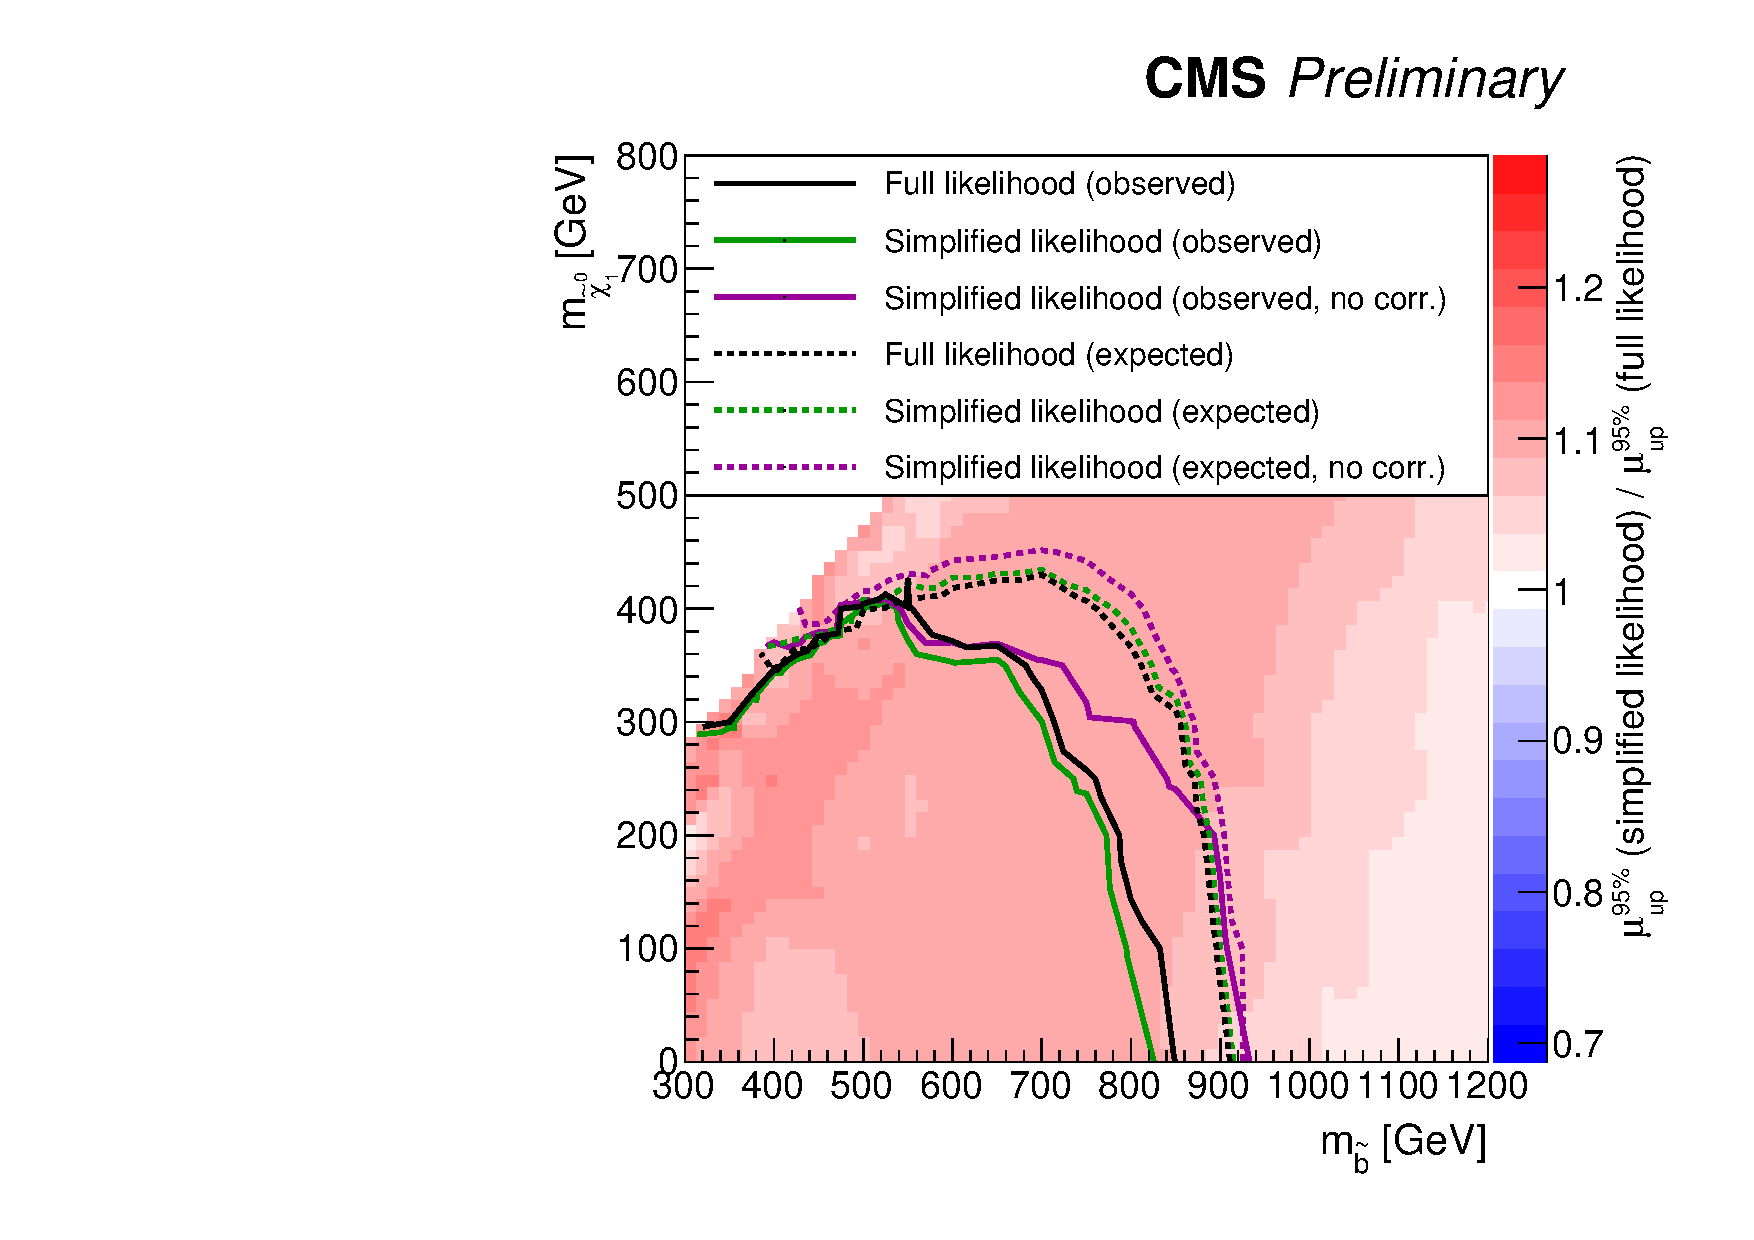
\includegraphics[width=0.45\textwidth]{Figures/simplifiedLikelihood/simpResults/full_T2bb_obs}}
   \caption{(a) The value of $q(r)$ for the \alphat search defined using the simplified likelihood using the full covariance matrix, assuming no correlations between the 
   background yields and defined using the full likelihood. (b) Expected and observed exclusion contours defined as 
   the boundary of the region where $r_{95} < 1$ for the \alphat search.
   The results are compared between the limits calculated using the full and the simplified likelihoods and the simplified likelihood assuming no correlations 
   between the background yields. The colour scale shows the ratio of $r_{95}$ calculated 
   using the simplified likelihood to the value using the full likelihood.}
   \label{fig:likelihoodscanAT} 
  \end{center}
\end{figure}

\section{Summary}

To re-interpret the \alphat~search requires the background model and associated
systematic uncertainties to be approximated. The categorisation may be
robustly simplified through the use of aggregated search regions while the simplified 
likelihood method uses a multivariate Gaussian to approximate the systematic uncertainties.
The simplified likelihood is shown to give comparable upper limits at 95\% confidence 
level for a representative signal model. These methods may be applied to a 
wide range of searches for new physics and a general treatment 
is presented in~\cite{simp-lik}.

